% Options for packages loaded elsewhere
\PassOptionsToPackage{unicode}{hyperref}
\PassOptionsToPackage{hyphens}{url}
\documentclass[
]{article}
\usepackage{xcolor}
\usepackage[margin=1in]{geometry}
\usepackage{amsmath,amssymb}
\setcounter{secnumdepth}{-\maxdimen} % remove section numbering
\usepackage{iftex}
\ifPDFTeX
  \usepackage[T1]{fontenc}
  \usepackage[utf8]{inputenc}
  \usepackage{textcomp} % provide euro and other symbols
\else % if luatex or xetex
  \usepackage{unicode-math} % this also loads fontspec
  \defaultfontfeatures{Scale=MatchLowercase}
  \defaultfontfeatures[\rmfamily]{Ligatures=TeX,Scale=1}
\fi
\usepackage{lmodern}
\ifPDFTeX\else
  % xetex/luatex font selection
\fi
% Use upquote if available, for straight quotes in verbatim environments
\IfFileExists{upquote.sty}{\usepackage{upquote}}{}
\IfFileExists{microtype.sty}{% use microtype if available
  \usepackage[]{microtype}
  \UseMicrotypeSet[protrusion]{basicmath} % disable protrusion for tt fonts
}{}
\makeatletter
\@ifundefined{KOMAClassName}{% if non-KOMA class
  \IfFileExists{parskip.sty}{%
    \usepackage{parskip}
  }{% else
    \setlength{\parindent}{0pt}
    \setlength{\parskip}{6pt plus 2pt minus 1pt}}
}{% if KOMA class
  \KOMAoptions{parskip=half}}
\makeatother
\usepackage{color}
\usepackage{fancyvrb}
\newcommand{\VerbBar}{|}
\newcommand{\VERB}{\Verb[commandchars=\\\{\}]}
\DefineVerbatimEnvironment{Highlighting}{Verbatim}{commandchars=\\\{\}}
% Add ',fontsize=\small' for more characters per line
\usepackage{framed}
\definecolor{shadecolor}{RGB}{248,248,248}
\newenvironment{Shaded}{\begin{snugshade}}{\end{snugshade}}
\newcommand{\AlertTok}[1]{\textcolor[rgb]{0.94,0.16,0.16}{#1}}
\newcommand{\AnnotationTok}[1]{\textcolor[rgb]{0.56,0.35,0.01}{\textbf{\textit{#1}}}}
\newcommand{\AttributeTok}[1]{\textcolor[rgb]{0.13,0.29,0.53}{#1}}
\newcommand{\BaseNTok}[1]{\textcolor[rgb]{0.00,0.00,0.81}{#1}}
\newcommand{\BuiltInTok}[1]{#1}
\newcommand{\CharTok}[1]{\textcolor[rgb]{0.31,0.60,0.02}{#1}}
\newcommand{\CommentTok}[1]{\textcolor[rgb]{0.56,0.35,0.01}{\textit{#1}}}
\newcommand{\CommentVarTok}[1]{\textcolor[rgb]{0.56,0.35,0.01}{\textbf{\textit{#1}}}}
\newcommand{\ConstantTok}[1]{\textcolor[rgb]{0.56,0.35,0.01}{#1}}
\newcommand{\ControlFlowTok}[1]{\textcolor[rgb]{0.13,0.29,0.53}{\textbf{#1}}}
\newcommand{\DataTypeTok}[1]{\textcolor[rgb]{0.13,0.29,0.53}{#1}}
\newcommand{\DecValTok}[1]{\textcolor[rgb]{0.00,0.00,0.81}{#1}}
\newcommand{\DocumentationTok}[1]{\textcolor[rgb]{0.56,0.35,0.01}{\textbf{\textit{#1}}}}
\newcommand{\ErrorTok}[1]{\textcolor[rgb]{0.64,0.00,0.00}{\textbf{#1}}}
\newcommand{\ExtensionTok}[1]{#1}
\newcommand{\FloatTok}[1]{\textcolor[rgb]{0.00,0.00,0.81}{#1}}
\newcommand{\FunctionTok}[1]{\textcolor[rgb]{0.13,0.29,0.53}{\textbf{#1}}}
\newcommand{\ImportTok}[1]{#1}
\newcommand{\InformationTok}[1]{\textcolor[rgb]{0.56,0.35,0.01}{\textbf{\textit{#1}}}}
\newcommand{\KeywordTok}[1]{\textcolor[rgb]{0.13,0.29,0.53}{\textbf{#1}}}
\newcommand{\NormalTok}[1]{#1}
\newcommand{\OperatorTok}[1]{\textcolor[rgb]{0.81,0.36,0.00}{\textbf{#1}}}
\newcommand{\OtherTok}[1]{\textcolor[rgb]{0.56,0.35,0.01}{#1}}
\newcommand{\PreprocessorTok}[1]{\textcolor[rgb]{0.56,0.35,0.01}{\textit{#1}}}
\newcommand{\RegionMarkerTok}[1]{#1}
\newcommand{\SpecialCharTok}[1]{\textcolor[rgb]{0.81,0.36,0.00}{\textbf{#1}}}
\newcommand{\SpecialStringTok}[1]{\textcolor[rgb]{0.31,0.60,0.02}{#1}}
\newcommand{\StringTok}[1]{\textcolor[rgb]{0.31,0.60,0.02}{#1}}
\newcommand{\VariableTok}[1]{\textcolor[rgb]{0.00,0.00,0.00}{#1}}
\newcommand{\VerbatimStringTok}[1]{\textcolor[rgb]{0.31,0.60,0.02}{#1}}
\newcommand{\WarningTok}[1]{\textcolor[rgb]{0.56,0.35,0.01}{\textbf{\textit{#1}}}}
\usepackage{graphicx}
\makeatletter
\newsavebox\pandoc@box
\newcommand*\pandocbounded[1]{% scales image to fit in text height/width
  \sbox\pandoc@box{#1}%
  \Gscale@div\@tempa{\textheight}{\dimexpr\ht\pandoc@box+\dp\pandoc@box\relax}%
  \Gscale@div\@tempb{\linewidth}{\wd\pandoc@box}%
  \ifdim\@tempb\p@<\@tempa\p@\let\@tempa\@tempb\fi% select the smaller of both
  \ifdim\@tempa\p@<\p@\scalebox{\@tempa}{\usebox\pandoc@box}%
  \else\usebox{\pandoc@box}%
  \fi%
}
% Set default figure placement to htbp
\def\fps@figure{htbp}
\makeatother
\setlength{\emergencystretch}{3em} % prevent overfull lines
\providecommand{\tightlist}{%
  \setlength{\itemsep}{0pt}\setlength{\parskip}{0pt}}
\usepackage{bookmark}
\IfFileExists{xurl.sty}{\usepackage{xurl}}{} % add URL line breaks if available
\urlstyle{same}
\hypersetup{
  pdftitle={Simulation Results},
  hidelinks,
  pdfcreator={LaTeX via pandoc}}

\title{Simulation Results}
\author{}
\date{\vspace{-2.5em}}

\begin{document}
\maketitle

\begin{Shaded}
\begin{Highlighting}[]
\FunctionTok{source}\NormalTok{(}\StringTok{"process{-}simulation{-}results.R"}\NormalTok{)}
\end{Highlighting}
\end{Shaded}

\begin{verbatim}
## -- Attaching core tidyverse packages ------------------------ tidyverse 2.0.0 --
## v dplyr     1.1.4     v readr     2.1.5
## v forcats   1.0.0     v stringr   1.5.1
## v ggplot2   3.5.2     v tibble    3.3.0
## v lubridate 1.9.3     v tidyr     1.3.1
## v purrr     1.0.4     
## -- Conflicts ------------------------------------------ tidyverse_conflicts() --
## x dplyr::filter() masks stats::filter()
## x dplyr::lag()    masks stats::lag()
## i Use the conflicted package (<http://conflicted.r-lib.org/>) to force all conflicts to become errors
\end{verbatim}

\begin{Shaded}
\begin{Highlighting}[]
\NormalTok{mu\_graph\_res\_main}\SpecialCharTok{$}\NormalTok{method }\OtherTok{=} \FunctionTok{fct}\NormalTok{(mu\_graph\_res\_main}\SpecialCharTok{$}\NormalTok{method, }\AttributeTok{levels =} \FunctionTok{c}\NormalTok{(}\StringTok{"Beta"}\NormalTok{,}\StringTok{"CHE{-}ISCW"}\NormalTok{,}\StringTok{"PET/PEESE"}\NormalTok{))}
\NormalTok{mu\_graph\_res\_ci\_main}\SpecialCharTok{$}\NormalTok{method }\OtherTok{=} \FunctionTok{fct}\NormalTok{(mu\_graph\_res\_ci\_main}\SpecialCharTok{$}\NormalTok{method, }\AttributeTok{levels =} \FunctionTok{c}\NormalTok{(}\StringTok{"Beta"}\NormalTok{,}\StringTok{"CHE{-}ISCW"}\NormalTok{,}\StringTok{"PET/PEESE"}\NormalTok{))}

\NormalTok{beta\_bias\_main }\OtherTok{\textless{}{-}}
\NormalTok{  mu\_graph\_res\_main }\SpecialCharTok{\%\textgreater{}\%}
  \FunctionTok{filter}\NormalTok{(model\_estimator }\SpecialCharTok{==} \StringTok{"beta\_CML"}\NormalTok{) }\SpecialCharTok{\%\textgreater{}\%}
  \FunctionTok{summarize}\NormalTok{(}
    \AttributeTok{max\_abs\_bias =} \FunctionTok{max}\NormalTok{(}\FunctionTok{abs}\NormalTok{(bias)),}
    \AttributeTok{min\_abs\_bias =} \FunctionTok{min}\NormalTok{(}\FunctionTok{abs}\NormalTok{(bias)),}
    \AttributeTok{max\_bias =} \FunctionTok{max}\NormalTok{(bias),}
    \AttributeTok{min\_bias =} \FunctionTok{min}\NormalTok{(bias)}
\NormalTok{  )}

\NormalTok{che\_bias\_main }\OtherTok{\textless{}{-}}
\NormalTok{  mu\_graph\_res\_main }\SpecialCharTok{\%\textgreater{}\%}
  \FunctionTok{filter}\NormalTok{(model\_estimator }\SpecialCharTok{==} \StringTok{"Comparison\_CHE{-}ISCW"}\NormalTok{) }\SpecialCharTok{\%\textgreater{}\%}
  \FunctionTok{summarize}\NormalTok{(}
    \AttributeTok{max\_abs\_bias =} \FunctionTok{max}\NormalTok{(}\FunctionTok{abs}\NormalTok{(bias)),}
    \AttributeTok{min\_abs\_bias =} \FunctionTok{min}\NormalTok{(}\FunctionTok{abs}\NormalTok{(bias)),}
    \AttributeTok{max\_bias =} \FunctionTok{max}\NormalTok{(bias),}
    \AttributeTok{min\_bias =} \FunctionTok{min}\NormalTok{(bias)}
\NormalTok{  )}

\NormalTok{pp\_bias\_main }\OtherTok{\textless{}{-}}
\NormalTok{  mu\_graph\_res\_main }\SpecialCharTok{\%\textgreater{}\%}
  \FunctionTok{filter}\NormalTok{(model\_estimator }\SpecialCharTok{==} \StringTok{"Comparison\_PET/PEESE"}\NormalTok{) }\SpecialCharTok{\%\textgreater{}\%}
  \FunctionTok{summarize}\NormalTok{(}
    \AttributeTok{max\_abs\_bias =} \FunctionTok{max}\NormalTok{(}\FunctionTok{abs}\NormalTok{(bias)),}
    \AttributeTok{min\_abs\_bias =} \FunctionTok{min}\NormalTok{(}\FunctionTok{abs}\NormalTok{(bias)),}
    \AttributeTok{max\_bias =} \FunctionTok{max}\NormalTok{(bias),}
    \AttributeTok{min\_bias =} \FunctionTok{min}\NormalTok{(bias)}
\NormalTok{  )}

\NormalTok{mu\_graph\_res\_miss}\SpecialCharTok{$}\NormalTok{method }\OtherTok{=} \FunctionTok{fct}\NormalTok{(mu\_graph\_res\_miss}\SpecialCharTok{$}\NormalTok{method, }\AttributeTok{levels =} \FunctionTok{c}\NormalTok{(}\StringTok{"Beta"}\NormalTok{,}\StringTok{"3PSM"}\NormalTok{,}\StringTok{"4PSM"}\NormalTok{))}
\NormalTok{mu\_graph\_res\_ci\_miss}\SpecialCharTok{$}\NormalTok{method }\OtherTok{=} \FunctionTok{fct}\NormalTok{(mu\_graph\_res\_ci\_miss}\SpecialCharTok{$}\NormalTok{method, }\AttributeTok{levels =} \FunctionTok{c}\NormalTok{(}\StringTok{"Beta"}\NormalTok{,}\StringTok{"3PSM"}\NormalTok{,}\StringTok{"4PSM"}\NormalTok{))}
\end{Highlighting}
\end{Shaded}

We organize our simulation results into two parts. First, we compare the
performance of the beta-function selection model to the CHE-ISCW and
PET/PEESE approaches. Specifically, we compare the bias and accuracy of
the average effect size, the coverage rates of 95\% confidence intervals
of the average effect size, and the estimation of the marginal variance
of the effect size distribution. Second, we compare the performance of
the beta-function selection model to the 3PSM and 4PSM step-function
models to assess the robustness of these models to misspecification of
the selection function.

\subsection{Beta-Function Selection Model Compared to CHE-ISCW and
PET/PEESE}\label{beta-function-selection-model-compared-to-che-iscw-and-petpeese}

\subsubsection{Average Effect Size}\label{average-effect-size}

The CHE-ISCW and PET/PEESE approaches had perfect convergence rates,
producing results for every replication in every condition. The
beta-function selection model exhibited very high convergence rates,
with an average rate of 99.6\%; the lowest convergence rates occurred
under conditions with the lowest degree of heterogeneity
\(\tau = 0.05\). Supplementary Figure @ref(fig:convergence-rates-main)
depicts the range of convergence rates of the beta-function selection
model.

\paragraph{Bias}\label{bias}

\begin{Shaded}
\begin{Highlighting}[]
\FunctionTok{ggplot}\NormalTok{(mu\_graph\_res\_main) }\SpecialCharTok{+} 
  \FunctionTok{aes}\NormalTok{(}\AttributeTok{x =}\NormalTok{ selection\_strength, }\AttributeTok{y =}\NormalTok{ bias, }\AttributeTok{color =}\NormalTok{ method, }\AttributeTok{fill =}\NormalTok{ method) }\SpecialCharTok{+}
  \FunctionTok{geom\_hline}\NormalTok{(}\AttributeTok{yintercept =} \DecValTok{0}\NormalTok{) }\SpecialCharTok{+}
  \FunctionTok{geom\_boxplot}\NormalTok{(}\AttributeTok{alpha =}\NormalTok{ .}\DecValTok{5}\NormalTok{, }\AttributeTok{coef =} \ConstantTok{Inf}\NormalTok{) }\SpecialCharTok{+}
  \FunctionTok{scale\_color\_brewer}\NormalTok{(}\AttributeTok{palette =} \StringTok{"Dark2"}\NormalTok{) }\SpecialCharTok{+}
  \FunctionTok{scale\_fill\_brewer}\NormalTok{(}\AttributeTok{palette =} \StringTok{"Dark2"}\NormalTok{) }\SpecialCharTok{+}
  \FunctionTok{scale\_x\_discrete}\NormalTok{(}\AttributeTok{labels =} \ControlFlowTok{function}\NormalTok{(x) stringr}\SpecialCharTok{::}\FunctionTok{str\_wrap}\NormalTok{(x, }\AttributeTok{width =} \DecValTok{3}\NormalTok{))}\SpecialCharTok{+}
  \FunctionTok{facet\_grid}\NormalTok{(}
\NormalTok{    tau }\SpecialCharTok{\textasciitilde{}}\NormalTok{ mean\_smd, }
    \AttributeTok{labeller =} \FunctionTok{label\_bquote}\NormalTok{(}
      \AttributeTok{rows =}\NormalTok{ tau }\SpecialCharTok{==}\NormalTok{ .(tau),}
      \AttributeTok{cols =}\NormalTok{ mu }\SpecialCharTok{==}\NormalTok{ .(mean\_smd)}
\NormalTok{    ),}
    \AttributeTok{scales =} \StringTok{"free\_y"}
\NormalTok{  ) }\SpecialCharTok{+}
  \FunctionTok{labs}\NormalTok{(}
    \AttributeTok{x =} \StringTok{"Selection probability"}\NormalTok{, }
    \AttributeTok{y =} \StringTok{"Bias"}\NormalTok{, }
    \AttributeTok{color =} \StringTok{"Method"}\NormalTok{,}
    \AttributeTok{fill =} \StringTok{"Method"}
\NormalTok{  ) }\SpecialCharTok{+} 
  \FunctionTok{theme\_bw}\NormalTok{() }\SpecialCharTok{+}
  \FunctionTok{theme}\NormalTok{(}\AttributeTok{legend.position =} \StringTok{"top"}\NormalTok{)}
\end{Highlighting}
\end{Shaded}

\begin{sidewaysfigure}
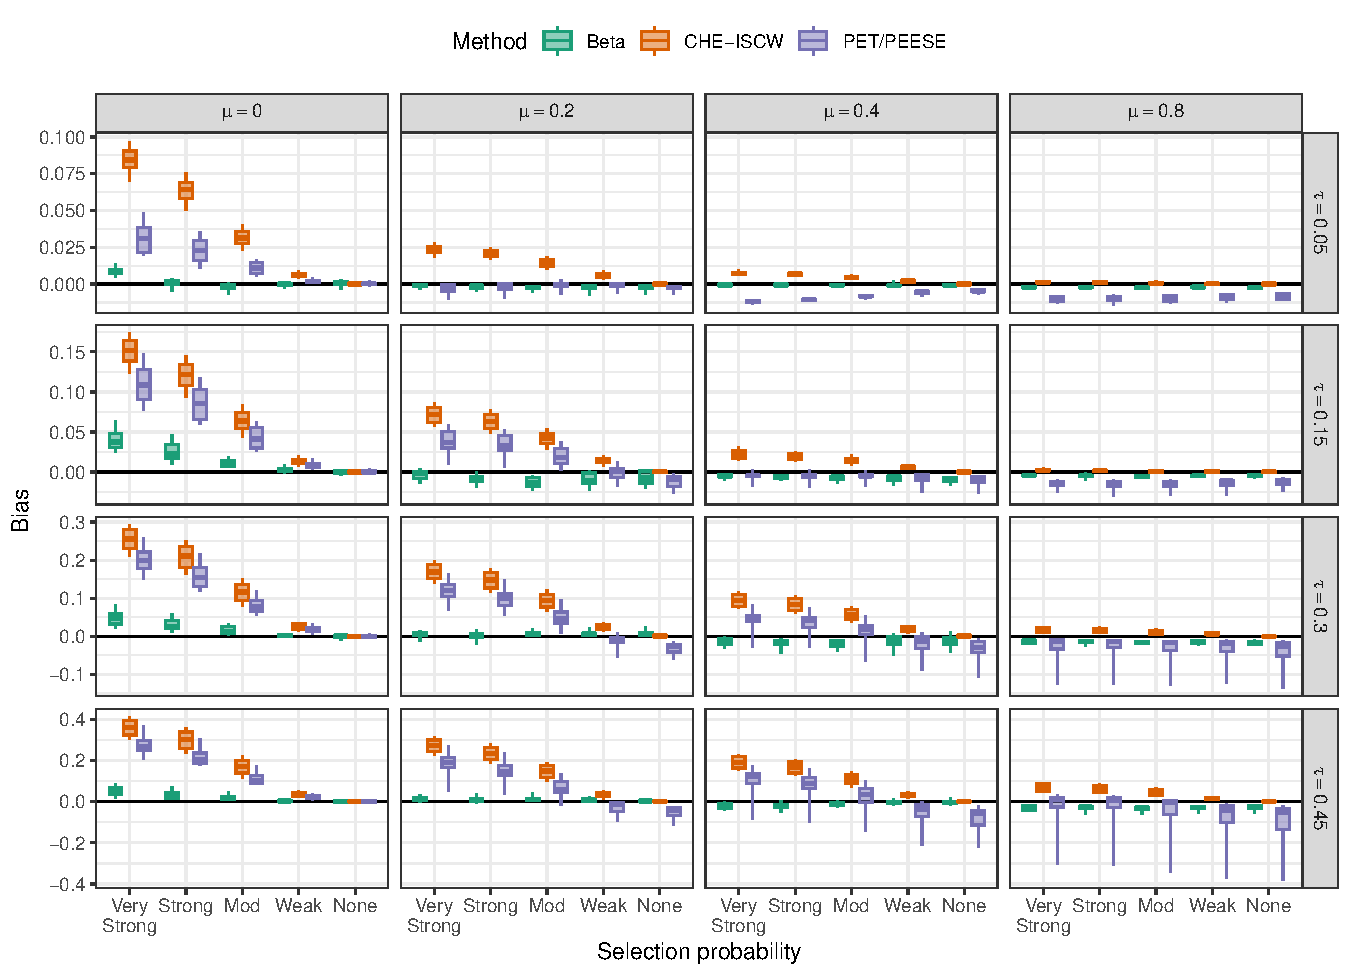
\includegraphics{simulation-results_files/figure-latex/mu-bias-main-1} \caption{Bias of the average effect size by method, selection probability, average SMD, and between-study heterogeneity}\label{fig:mu-bias-main}
\end{sidewaysfigure}

Figure (\textbf{ref?})(fig:mu-bias-main) shows the bias for each method
of estimating the average effect size (vertical axis) as a function of
selective reporting strength (horizontal axis), average effect size
(grid column), and between-study heterogeneity (\(\tau\), grid row).
Each box plot summarizes variation in bias across the remaining
simulation factors: the heterogeneity ratio, the correlation between
effect size estimates, and the number of observed studies. Note that the
vertical axis scale differs by grid row, reflecting how some methods'
bias is more sensitive to the level of heterogeneity.

The beta-function selection model has negligible to small bias across
all conditions, ranging from -0.06 to 0.09. Its bias was essentially
zero for all conditions when the average effect size is non-zero or when
selective reporting is weak or absent. Bias was largest when selective
reporting is very strong, average effect size is zero, and heterogeneity
is large.

In contrast, bias for the comparison methods ranged from 0 to 0.41 for
CHE-ISCW and -0.38 to 0.37 for PET/PEESE. Both methods are generally
biased when selective reporting is not absent. For CHE-ISCW, which does
not directly adjust for selective reporting, bias was closest to zero
when average effect size is large \((\mu = 0.8)\) and heterogeneity is
low \((\tau \leq 0.15)\). For PET/PEESE, which uses a regression
adjustment to account for possible selective reporting, bias was closest
to zero when average effect size is moderate \((\mu = 0.4)\) and
heterogeneity is low \((\tau = 0.15)\). For both comparison methods,
bias grows stronger when selection is stronger, when average effect size
is smaller, and when heterogeneity is larger; however, bias is generally
less pronounced for PET/PEESE than CHE-ISCW.

\paragraph{Scaled RMSE}\label{scaled-rmse}

\begin{Shaded}
\begin{Highlighting}[]
\FunctionTok{ggplot}\NormalTok{(mu\_graph\_res\_main) }\SpecialCharTok{+} 
  \FunctionTok{aes}\NormalTok{(}\AttributeTok{x =}\NormalTok{ selection\_strength, }\AttributeTok{y =}\NormalTok{ scrmse, }\AttributeTok{color =}\NormalTok{ method, }\AttributeTok{fill =}\NormalTok{ method) }\SpecialCharTok{+}
  \FunctionTok{geom\_hline}\NormalTok{(}\AttributeTok{yintercept =} \DecValTok{0}\NormalTok{) }\SpecialCharTok{+}
  \FunctionTok{geom\_boxplot}\NormalTok{(}\AttributeTok{alpha =}\NormalTok{ .}\DecValTok{5}\NormalTok{, }\AttributeTok{coef =} \ConstantTok{Inf}\NormalTok{) }\SpecialCharTok{+}
  \FunctionTok{scale\_color\_brewer}\NormalTok{(}\AttributeTok{palette =} \StringTok{"Dark2"}\NormalTok{) }\SpecialCharTok{+}
  \FunctionTok{scale\_fill\_brewer}\NormalTok{(}\AttributeTok{palette =} \StringTok{"Dark2"}\NormalTok{) }\SpecialCharTok{+}
  \FunctionTok{scale\_x\_discrete}\NormalTok{(}\AttributeTok{labels =} \ControlFlowTok{function}\NormalTok{(x) stringr}\SpecialCharTok{::}\FunctionTok{str\_wrap}\NormalTok{(x, }\AttributeTok{width =} \DecValTok{3}\NormalTok{))}\SpecialCharTok{+}
  \FunctionTok{facet\_grid}\NormalTok{(}
\NormalTok{    tau }\SpecialCharTok{\textasciitilde{}}\NormalTok{ mean\_smd, }
    \AttributeTok{labeller =} \FunctionTok{label\_bquote}\NormalTok{(}
      \AttributeTok{rows =}\NormalTok{ tau }\SpecialCharTok{==}\NormalTok{ .(tau),}
      \AttributeTok{cols =}\NormalTok{ mu }\SpecialCharTok{==}\NormalTok{ .(mean\_smd)}
\NormalTok{    ),}
    \AttributeTok{scales =} \StringTok{"free\_y"}
\NormalTok{  ) }\SpecialCharTok{+}
  \FunctionTok{labs}\NormalTok{(}
    \AttributeTok{x =} \StringTok{"Selection probability"}\NormalTok{, }
    \AttributeTok{y =} \StringTok{"Scaled Root Mean{-}Squared Error"}\NormalTok{, }
    \AttributeTok{color =} \StringTok{"Method"}\NormalTok{,}
    \AttributeTok{fill =} \StringTok{"Method"}
\NormalTok{  ) }\SpecialCharTok{+} 
  \FunctionTok{theme\_bw}\NormalTok{() }\SpecialCharTok{+}
  \FunctionTok{theme}\NormalTok{(}\AttributeTok{legend.position =} \StringTok{"top"}\NormalTok{)}
\end{Highlighting}
\end{Shaded}

\begin{sidewaysfigure}
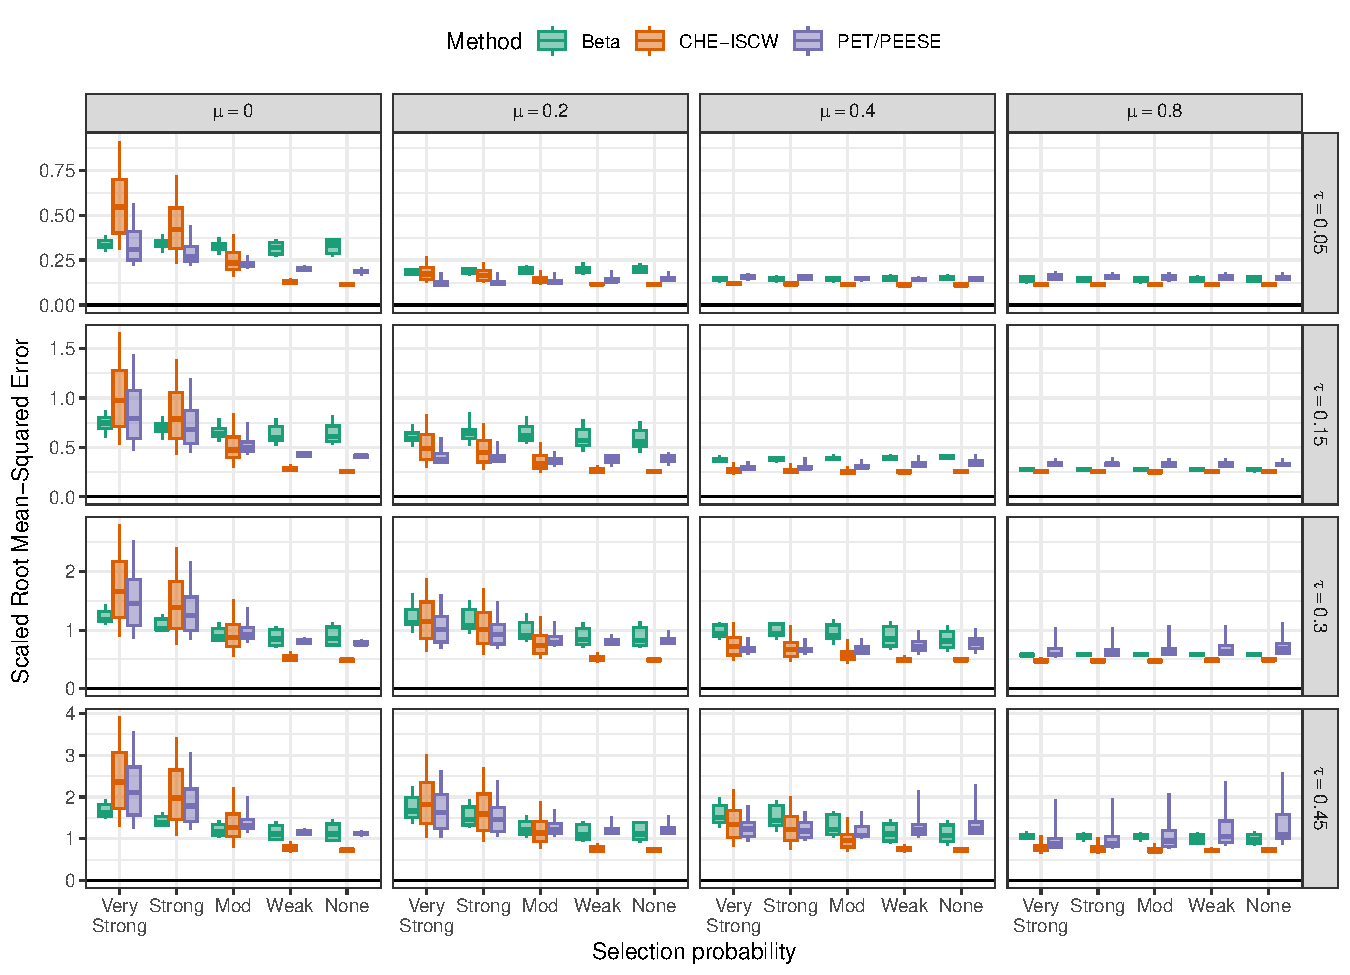
\includegraphics{simulation-results_files/figure-latex/mu-rmse-main-1} \caption{Scaled root mean-squared error of the average effect size by method, selection probability, average SMD, and between-study heterogeneity}\label{fig:mu-rmse-main}
\end{sidewaysfigure}

Scaled RMSE captures both bias and variability, providing an overall
measure of inaccuracy. Figure (\textbf{ref?})(fig:mu-rmse-main),
constructed in the same format as Figure
(\textbf{ref?})(fig:mu-bias-main), shows the scaled RMSE for each method
of estimating the average effect size. Additional detail is provided in
Figures (\textbf{ref?})(fig:rmse-CHE-Beta-main) and
(\textbf{ref?})(fig:rmse-PET-Beta-main) in Appendix
(\textbf{ref?})(mu-simulation-results-main), which plot the ratio of
RMSEs for each pair of methods to compare their relative accuracy.

Taken together, the figures indicate that no single method achieves the
lowest RMSE across all conditions. Instead, each method reflects
different bias--variance trade-offs. The beta-function selection model
generally outperforms the others---achieving lower RMSE---when selective
reporting is strong or very strong, average effect size is small
\((\mu \leq 0.2)\), and heterogeneity is moderate to large
\((\tau \geq 0.3)\). CHE-ISCW consistently has the lowest RMSE when
selective reporting is weak or absent. PET/PEESE performs best when
selective reporting is strong to very strong, average effect is small
\((\mu \leq 0.2)\), and heterogeneity is low \((\tau \leq 0.15)\).

These bias--variance trade-offs stem from the fact that CHE-ISCW, which
does not explicitly adjust for selective reporting, is more prone to
bias when selection is present. In contrast, the beta-function selection
model tends to produce smaller biases under such conditions. However,
when selective reporting is weak or absent, CHE-ISCW is more precise
than the methods that adjust for selective reporting (i.e., the
beta-function selection model and PET/PEESE). Under those conditions,
the added variability introduced by estimating a selection model or
PET/PEESE adjustment outweighs the minimal reduction in bias they
provide.

\paragraph{Confidence Interval
Coverage}\label{confidence-interval-coverage}

\begin{Shaded}
\begin{Highlighting}[]
\NormalTok{mu\_graph\_res\_ci\_main }\SpecialCharTok{\%\textgreater{}\%}
  \FunctionTok{filter}\NormalTok{(}
\NormalTok{    CI\_type }\SpecialCharTok{\%in\%} \FunctionTok{c}\NormalTok{(}\StringTok{"large{-}sample"}\NormalTok{)}
\NormalTok{  ) }\SpecialCharTok{\%\textgreater{}\%}
  \FunctionTok{ggplot}\NormalTok{(}\FunctionTok{aes}\NormalTok{(}\AttributeTok{x =}\NormalTok{ J, }\AttributeTok{y =}\NormalTok{ coverage, }\AttributeTok{color =}\NormalTok{ method, }\AttributeTok{fill =}\NormalTok{ method)) }\SpecialCharTok{+}
  \FunctionTok{geom\_boxplot}\NormalTok{(}\AttributeTok{alpha =}\NormalTok{ .}\DecValTok{5}\NormalTok{, }\AttributeTok{coef =} \ConstantTok{Inf}\NormalTok{) }\SpecialCharTok{+}
  \FunctionTok{geom\_hline}\NormalTok{(}\AttributeTok{yintercept =} \FloatTok{0.95}\NormalTok{, }\AttributeTok{linetype =} \StringTok{"dashed"}\NormalTok{) }\SpecialCharTok{+}
  \FunctionTok{coord\_cartesian}\NormalTok{(}\AttributeTok{ylim =} \FunctionTok{c}\NormalTok{(}\FloatTok{0.5}\NormalTok{, }\FloatTok{1.0}\NormalTok{)) }\SpecialCharTok{+} 
  \FunctionTok{scale\_y\_continuous}\NormalTok{(}\AttributeTok{expand =} \FunctionTok{expansion}\NormalTok{(}\FunctionTok{c}\NormalTok{(}\DecValTok{0}\NormalTok{,}\DecValTok{0}\NormalTok{),}\FunctionTok{c}\NormalTok{(}\FloatTok{0.02}\NormalTok{,}\DecValTok{0}\NormalTok{))) }\SpecialCharTok{+} 
  \FunctionTok{scale\_color\_brewer}\NormalTok{(}\AttributeTok{palette =} \StringTok{"Dark2"}\NormalTok{) }\SpecialCharTok{+}
  \FunctionTok{scale\_fill\_brewer}\NormalTok{(}\AttributeTok{palette =} \StringTok{"Dark2"}\NormalTok{) }\SpecialCharTok{+}
  \FunctionTok{facet\_grid}\NormalTok{(}
\NormalTok{    tau }\SpecialCharTok{\textasciitilde{}}\NormalTok{ mean\_smd, }
    \AttributeTok{labeller =} \FunctionTok{label\_bquote}\NormalTok{(}
      \AttributeTok{rows =}\NormalTok{ tau }\SpecialCharTok{==}\NormalTok{ .(tau),}
      \AttributeTok{cols =}\NormalTok{ mu }\SpecialCharTok{==}\NormalTok{ .(mean\_smd)}
\NormalTok{    ),}
    \AttributeTok{scales =} \StringTok{"free\_y"}
\NormalTok{  ) }\SpecialCharTok{+}
  \FunctionTok{labs}\NormalTok{(}
    \AttributeTok{x =} \StringTok{"Number of studies (J)"}\NormalTok{, }
    \AttributeTok{y =} \StringTok{"Coverage rate"}\NormalTok{, }
    \AttributeTok{color =} \StringTok{"Method"}\NormalTok{,}
    \AttributeTok{fill =} \StringTok{"Method"}
\NormalTok{  ) }\SpecialCharTok{+} 
  \FunctionTok{theme\_bw}\NormalTok{() }\SpecialCharTok{+}
  \FunctionTok{theme}\NormalTok{(}\AttributeTok{legend.position =} \StringTok{"top"}\NormalTok{)}
\end{Highlighting}
\end{Shaded}

\begin{sidewaysfigure}
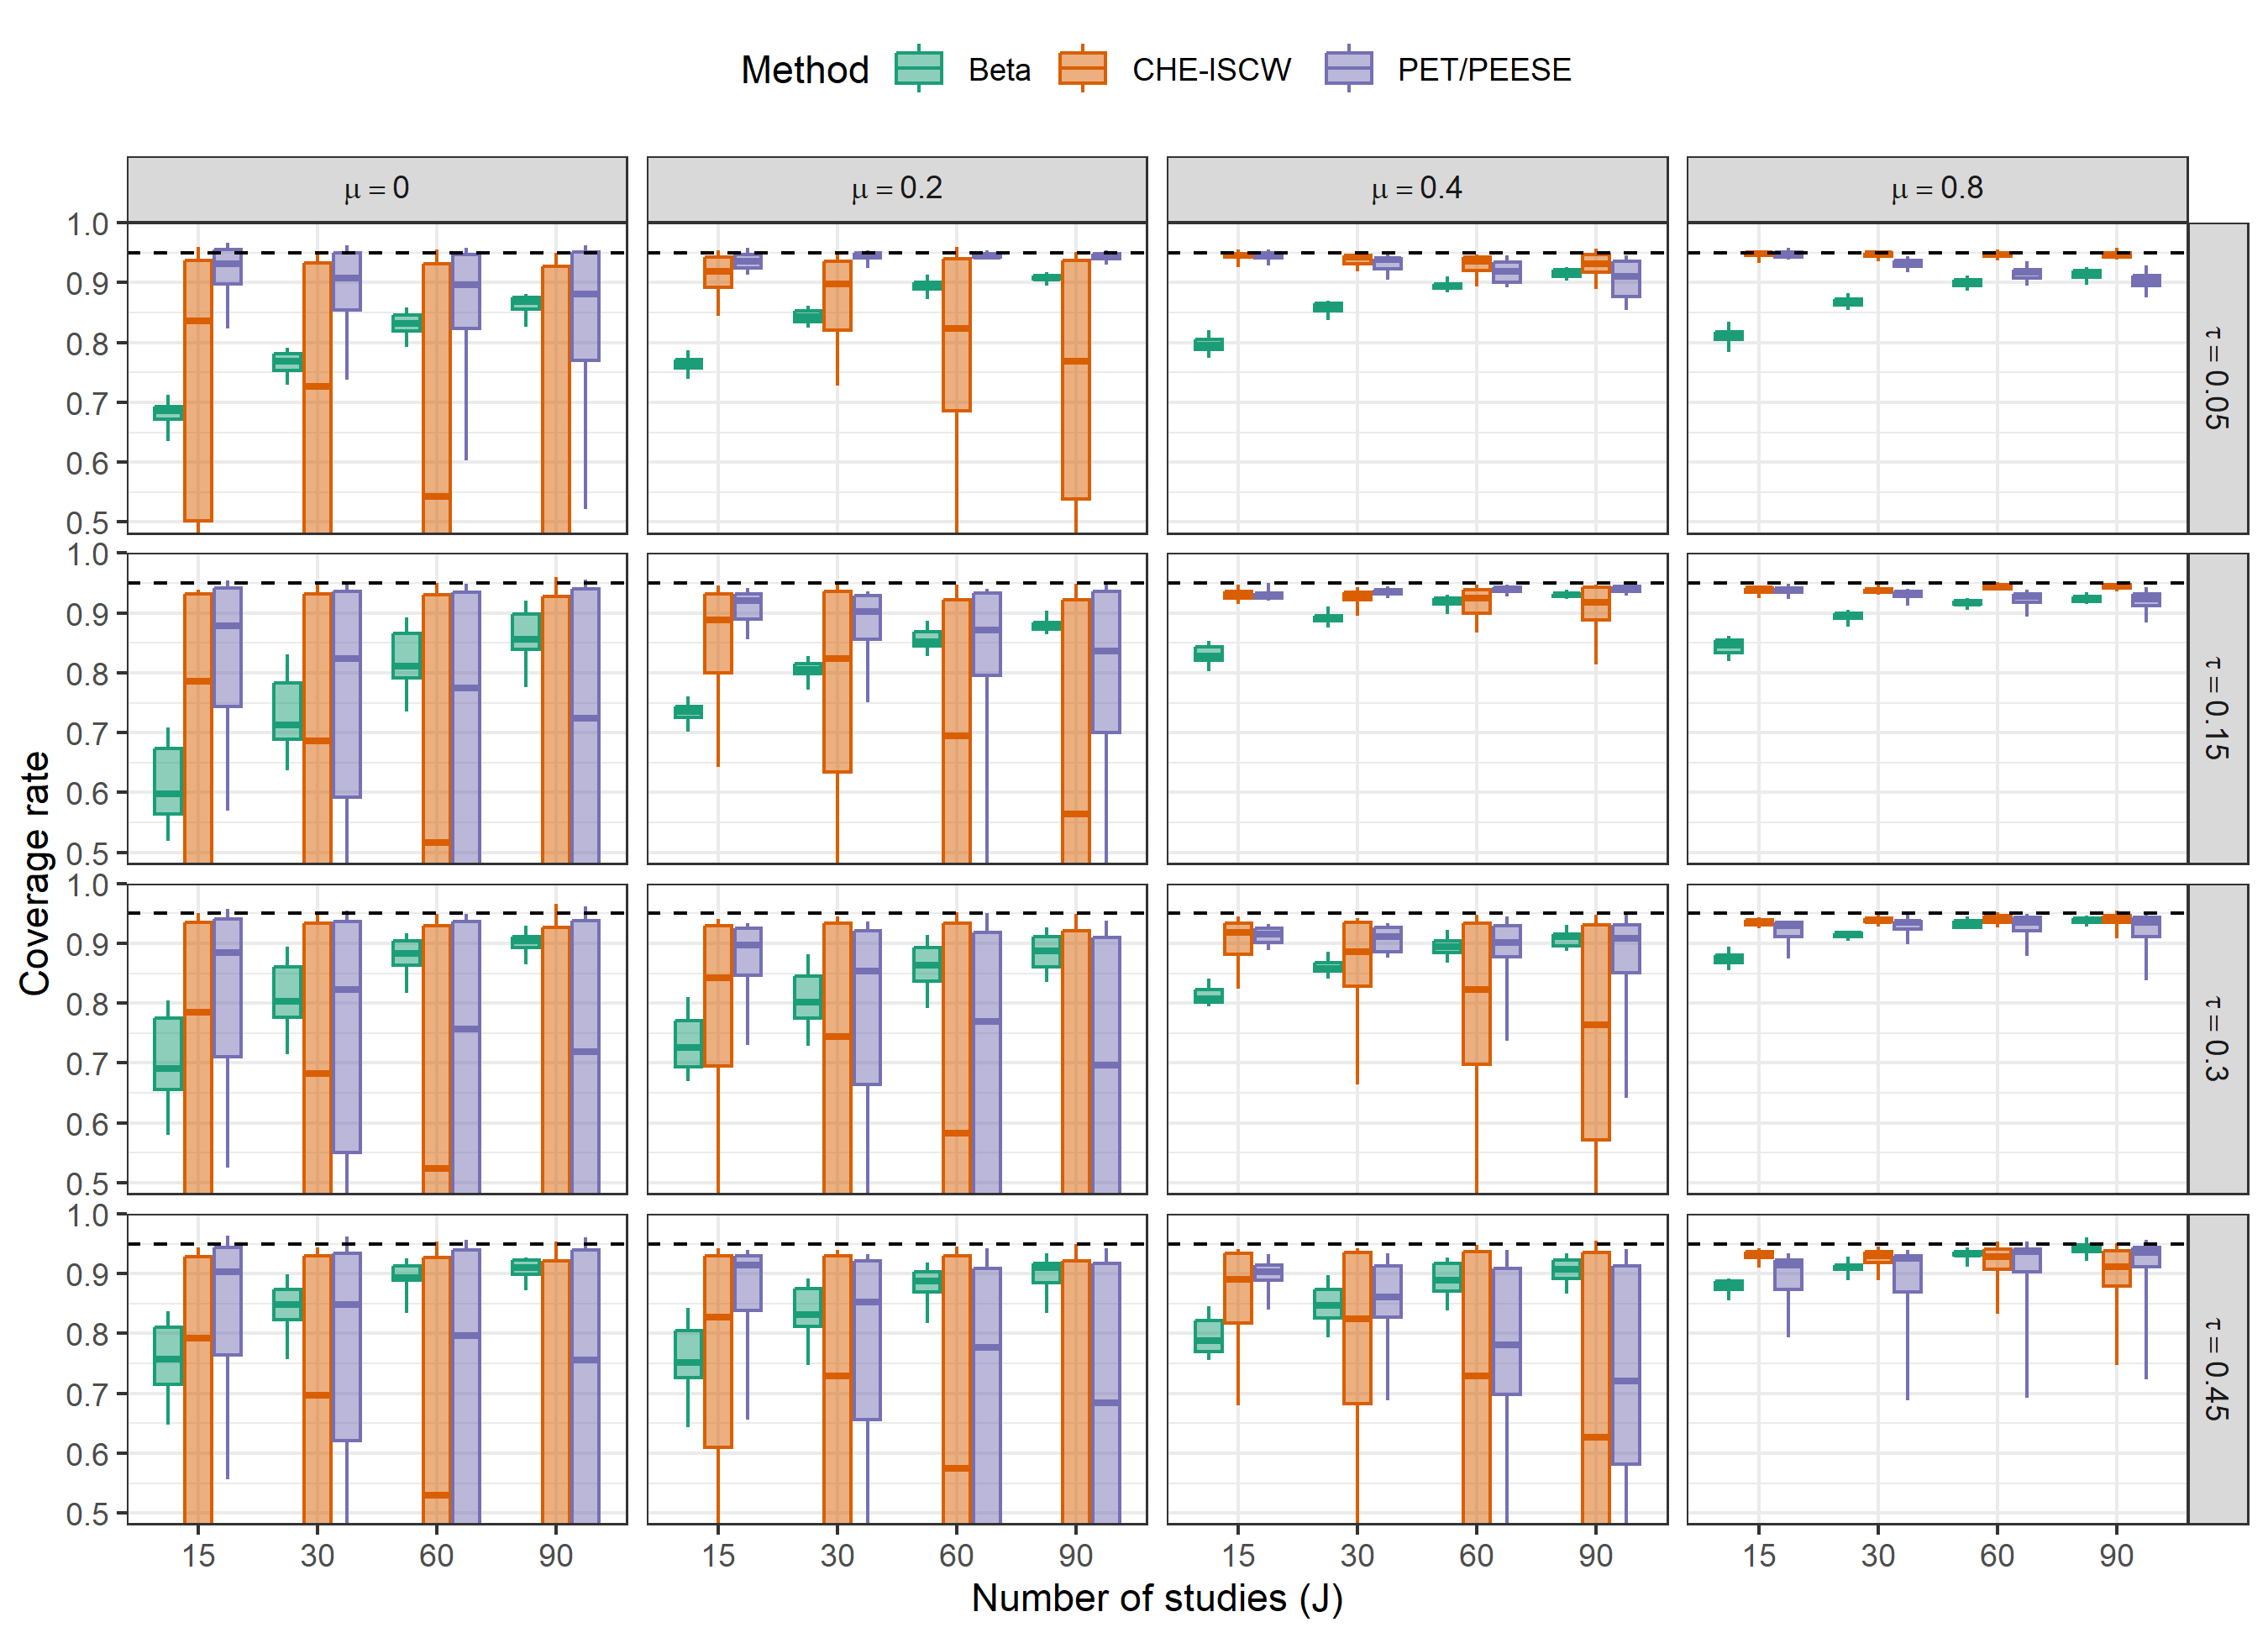
\includegraphics{simulation-results_files/figure-latex/comparison-coverage-main-1} \caption{Coverage levels of confidence intervals for the average effect size based on cluster-robust variance approximations, by method, number of studies, average SMD, and between-study heterogeneity. Dashed lines correspond to the nominal confidence level of 0.95. Coverage rates of the CHE-ISCW and PET/PEESE intervals are not depicted when they fall below 0.5}\label{fig:comparison-coverage-main}
\end{sidewaysfigure}

Figure @ref(fig:comparison-coverage-main) shows the coverage rates of
95\% confidence intervals based on large-sample cluster-robust variance
approximations for the three methods.\footnote{Note that the vertical
  axis of Figure @ref(fig:comparison-coverage-main) is restricted to the
  range {[}0.5, 1.0{]}, and coverage rates of the intervals based on
  CHE-ISCW and PET/PEESE are not depicted when they fall below 0.5.
  Supplementary Figure @ref(fig:comparison-coverage-full-main) depicts
  the full range of coverage rates.} Across most conditions, coverage
rates fall below the nominal rate of 0.95 for all methods. However, the
beta-function selection model generally achieves higher coverage than
the comparison methods, particularly when heterogeneity is moderate to
large (\(\tau \geq 0.3\)), or when heterogeneity is small
(\(\tau \leq 0.15\)), average effect size is small (\(\mu \leq 0.2\)),
and number of studies (\(J\)) is 60 or more.

In contrast, the confidence intervals produced by the comparison methods
are often severely miscalibrated. When CHE-ISCW and PET/PEESE are biased
due to selective reporting, their intervals tend to be centered away
from the true parameter. As a result, as the number of studies
increases, the standard errors of the average effect size
estimate-----and thus the interval widths-----shrink, causing coverage
rates to decline sharply, in some cases approaching zero.

\begin{Shaded}
\begin{Highlighting}[]
\NormalTok{mu\_graph\_res\_ci\_main }\SpecialCharTok{\%\textgreater{}\%}
  \FunctionTok{filter}\NormalTok{(}
\NormalTok{    bootstrap\_condition }\SpecialCharTok{==} \StringTok{"bootstrap"}\NormalTok{,}
\NormalTok{    estimator }\SpecialCharTok{\%in\%} \FunctionTok{c}\NormalTok{(}\StringTok{"CML"}\NormalTok{)}
    \CommentTok{\#estimator \%in\% c("CML"),}
    \CommentTok{\#CI\_type \%in\% c("large{-}sample","percentile")}
\NormalTok{  ) }\SpecialCharTok{\%\textgreater{}\%}
  \FunctionTok{ggplot}\NormalTok{(}\FunctionTok{aes}\NormalTok{(}\AttributeTok{x =}\NormalTok{ J, }\AttributeTok{y =}\NormalTok{ coverage, }\AttributeTok{color =}\NormalTok{ CI\_boot\_method, }\AttributeTok{fill =}\NormalTok{ CI\_boot\_method)) }\SpecialCharTok{+}
  \FunctionTok{geom\_boxplot}\NormalTok{(}\AttributeTok{alpha =}\NormalTok{ .}\DecValTok{5}\NormalTok{, }\AttributeTok{coef =} \ConstantTok{Inf}\NormalTok{) }\SpecialCharTok{+}
  \FunctionTok{geom\_hline}\NormalTok{(}\AttributeTok{yintercept =} \FloatTok{0.95}\NormalTok{, }\AttributeTok{linetype =} \StringTok{"dashed"}\NormalTok{) }\SpecialCharTok{+}
  \CommentTok{\#scale\_y\_continuous(limits = c(0.55, 1.0), breaks = seq(0.55,1.0,0.05), expand = expansion(0,0)) +}
  \FunctionTok{scale\_y\_continuous}\NormalTok{(}\AttributeTok{limits =} \FunctionTok{c}\NormalTok{(}\FloatTok{0.55}\NormalTok{, }\FloatTok{1.0}\NormalTok{)) }\SpecialCharTok{+}
  \FunctionTok{scale\_color\_brewer}\NormalTok{(}\AttributeTok{palette =} \StringTok{"Dark2"}\NormalTok{) }\SpecialCharTok{+}
  \FunctionTok{scale\_fill\_brewer}\NormalTok{(}\AttributeTok{palette =} \StringTok{"Dark2"}\NormalTok{) }\SpecialCharTok{+}
  \FunctionTok{facet\_grid}\NormalTok{(}
\NormalTok{    tau }\SpecialCharTok{\textasciitilde{}}\NormalTok{ mean\_smd,}
    \AttributeTok{labeller =} \FunctionTok{label\_bquote}\NormalTok{(}
      \AttributeTok{rows =}\NormalTok{ tau }\SpecialCharTok{==}\NormalTok{ .(tau),}
      \AttributeTok{cols =}\NormalTok{ mu }\SpecialCharTok{==}\NormalTok{ .(mean\_smd)}
\NormalTok{    ),}
    \AttributeTok{scales =} \StringTok{"free\_y"}
\NormalTok{  ) }\SpecialCharTok{+}
  \FunctionTok{labs}\NormalTok{(}
    \AttributeTok{x =} \StringTok{"Number of studies (J)"}\NormalTok{,}
    \AttributeTok{y =} \StringTok{"Coverage rate"}\NormalTok{,}
    \AttributeTok{color =} \StringTok{"Bootstrap Method"}\NormalTok{,}
    \AttributeTok{fill =} \StringTok{"Bootstrap Method"}
\NormalTok{  ) }\SpecialCharTok{+}
  \FunctionTok{theme\_bw}\NormalTok{() }\SpecialCharTok{+}
  \FunctionTok{theme}\NormalTok{(}\AttributeTok{legend.position =} \StringTok{"top"}\NormalTok{)}
\end{Highlighting}
\end{Shaded}

\begin{verbatim}
## Warning: Computation failed in `stat_boxplot()`.
## Caused by error in `if (any(outliers)) ...`:
## ! missing value where TRUE/FALSE needed
\end{verbatim}

\begin{sidewaysfigure}
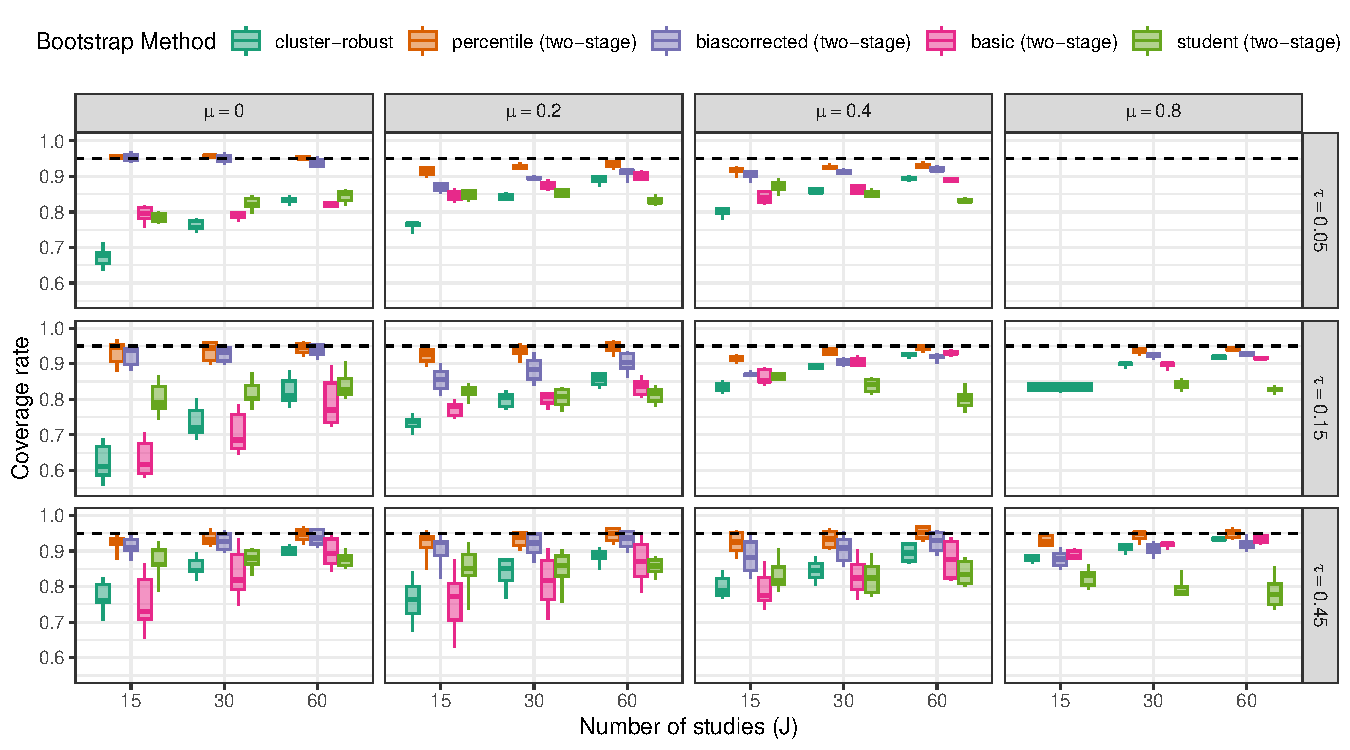
\includegraphics{simulation-results_files/figure-latex/Beta-coverage-main-1} \caption{Coverage levels of confidence intervals for the average effect size estimated using the beta-function selection model, by bootstrap method, number of studies, average SMD, and between-study heterogeneity. Dashed lines correspond to the nominal confidence level of 0.95.}\label{fig:Beta-coverage-main}
\end{sidewaysfigure}

Figure @ref(fig:Beta-coverage-main) depicts the coverage rates of 95\%
confidence intervals for the average effect size estimated using the
beta-function selection model, comparing intervals based on the
large-sample cluster-robust variance method to four two-stage
bootstrapping methods (percentile, basic, studentized, and
bias-corrected-and-accelerated). Due to the computational demands of
bootstrapping, we evaluated the bootstrap confidence intervals under a
more limited range of data-generating conditions, including a maximum
sample size of \(J = 60\). Although no method achieves exact nominal
coverage across all conditions, the percentile, studentized, and
bias-corrected-and-accelerated bootstrap intervals consistently yield
coverage rates comparable to-----or better than-----those based on the
large-sample cluster-robust variance method. Among these, the percentile
bootstrap intervals performed best, achieving coverage above 90\% in
nearly all conditions examined.

\subsection{Beta-Function Selection Model Compared to 3PSM and 4PSM
Step-Function Selection
Models}\label{beta-function-selection-model-compared-to-3psm-and-4psm-step-function-selection-models}

\subsubsection{Average Effect Size}\label{average-effect-size-1}

Convergence rates were higher for the step-function selection models
than for the beta-function selection model. Both the 3PSM and 4PSM
models had convergence rates of 99\% and above across all 1,280
conditions, while the beta-function selection model had convergence
rates below 99\% for 40 conditions.

\paragraph{Bias}\label{bias-1}

\begin{Shaded}
\begin{Highlighting}[]
\FunctionTok{ggplot}\NormalTok{(mu\_graph\_res\_miss) }\SpecialCharTok{+} 
  \FunctionTok{aes}\NormalTok{(}\AttributeTok{x =}\NormalTok{ selection\_strength, }\AttributeTok{y =}\NormalTok{ bias, }\AttributeTok{color =}\NormalTok{ method, }\AttributeTok{fill =}\NormalTok{ method) }\SpecialCharTok{+}
  \FunctionTok{geom\_hline}\NormalTok{(}\AttributeTok{yintercept =} \DecValTok{0}\NormalTok{) }\SpecialCharTok{+}
  \FunctionTok{geom\_boxplot}\NormalTok{(}\AttributeTok{alpha =}\NormalTok{ .}\DecValTok{5}\NormalTok{, }\AttributeTok{coef =} \ConstantTok{Inf}\NormalTok{) }\SpecialCharTok{+}
  \FunctionTok{scale\_color\_brewer}\NormalTok{(}\AttributeTok{palette =} \StringTok{"Dark2"}\NormalTok{) }\SpecialCharTok{+}
  \FunctionTok{scale\_fill\_brewer}\NormalTok{(}\AttributeTok{palette =} \StringTok{"Dark2"}\NormalTok{) }\SpecialCharTok{+}
  \FunctionTok{scale\_x\_discrete}\NormalTok{(}\AttributeTok{labels =} \ControlFlowTok{function}\NormalTok{(x) stringr}\SpecialCharTok{::}\FunctionTok{str\_wrap}\NormalTok{(x, }\AttributeTok{width =} \DecValTok{3}\NormalTok{))}\SpecialCharTok{+}
  \FunctionTok{facet\_grid}\NormalTok{(}
\NormalTok{    tau }\SpecialCharTok{\textasciitilde{}}\NormalTok{ mean\_smd, }
    \AttributeTok{labeller =} \FunctionTok{label\_bquote}\NormalTok{(}
      \AttributeTok{rows =}\NormalTok{ tau }\SpecialCharTok{==}\NormalTok{ .(tau),}
      \AttributeTok{cols =}\NormalTok{ mu }\SpecialCharTok{==}\NormalTok{ .(mean\_smd)}
\NormalTok{    ),}
    \AttributeTok{scales =} \StringTok{"free\_y"}
\NormalTok{  ) }\SpecialCharTok{+}
  \FunctionTok{labs}\NormalTok{(}
    \AttributeTok{x =} \StringTok{"Selection probability"}\NormalTok{, }
    \AttributeTok{y =} \StringTok{"Bias"}\NormalTok{, }
    \AttributeTok{color =} \StringTok{"Method"}\NormalTok{,}
    \AttributeTok{fill =} \StringTok{"Method"}
\NormalTok{  ) }\SpecialCharTok{+} 
  \FunctionTok{theme\_bw}\NormalTok{() }\SpecialCharTok{+}
  \FunctionTok{theme}\NormalTok{(}\AttributeTok{legend.position =} \StringTok{"top"}\NormalTok{)}
\end{Highlighting}
\end{Shaded}

\begin{sidewaysfigure}
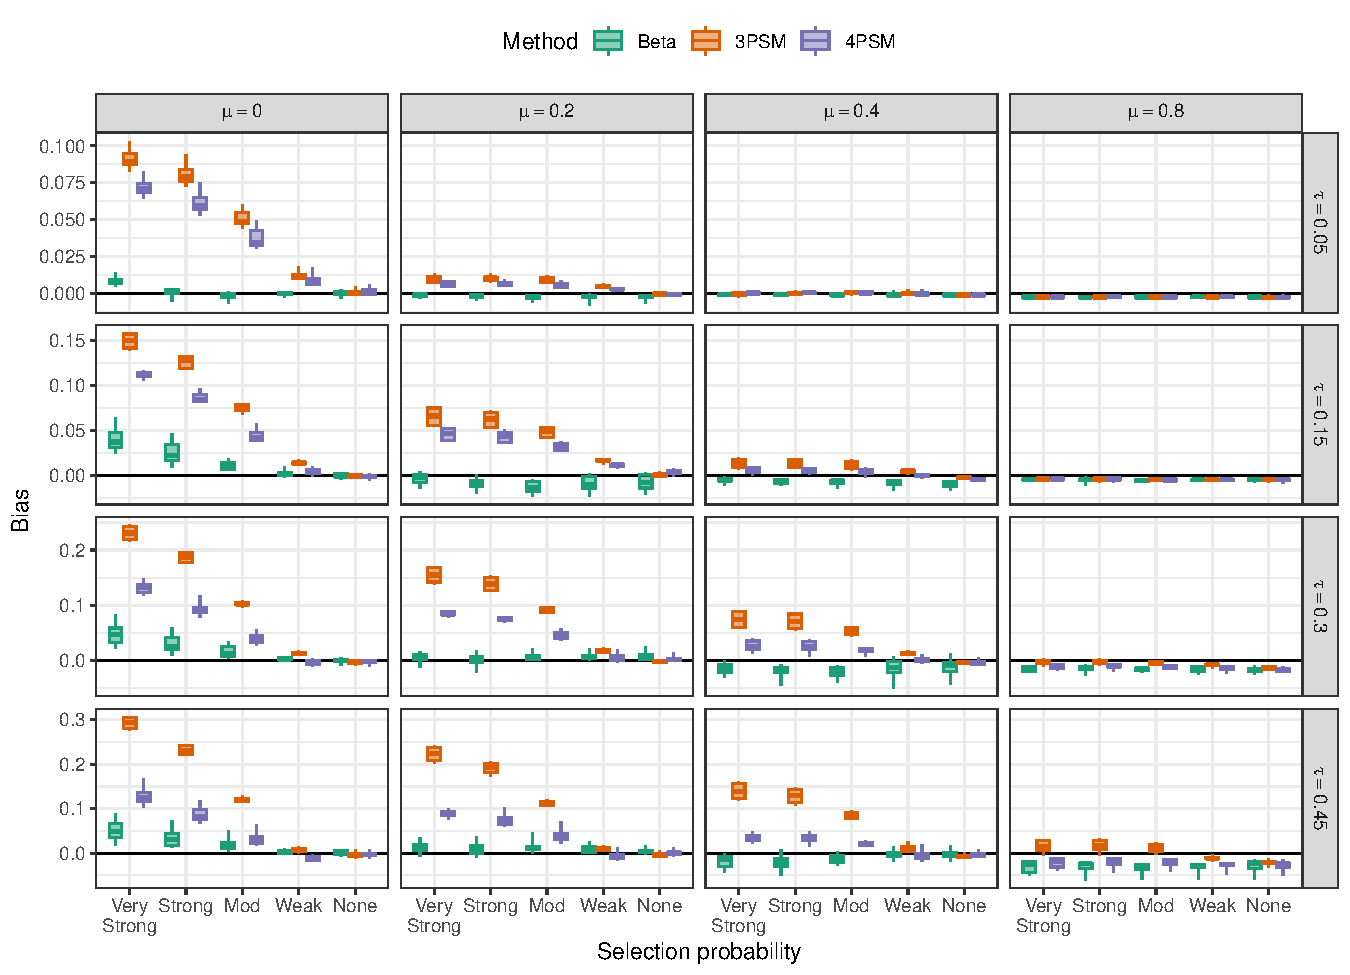
\includegraphics{simulation-results_files/figure-latex/mu-bias-miss-1} \caption{Bias of the average effect size by method, selection probability, average SMD, and between-study heterogeneity}\label{fig:mu-bias-miss}
\end{sidewaysfigure}

Figure (\textbf{ref?})(fig:mu-bias-miss) displays the bias for the three
selection models. Across most conditions, bias is consistently closer to
zero when the average effect size is estimated using the beta-function
selection model compared to the step-function selection models. Among
the step-function selection models, 4PSM generally outperforms 3PSM,
though both are more prone to bias when the selection process is
misspecified. The main exception occurs when average effect size is
moderate to large \((\mu \geq 0.4)\) and heterogeneity is low
\((\tau \leq 0.15)\), in which case all three models exhibit essentially
zero bias. This pattern is consistent with the fact that the data were
generated under a beta-function selection process and suggests that the
step-function selection models, particularly 3PSM, are not robust to
misspecification of the selection mechanism-----especially when
selective reporting is moderate to strong or when average effect is not
large \((\mu < 0.8)\).

\paragraph{Scaled RMSE}\label{scaled-rmse-1}

\begin{Shaded}
\begin{Highlighting}[]
\FunctionTok{ggplot}\NormalTok{(mu\_graph\_res\_miss) }\SpecialCharTok{+} 
  \FunctionTok{aes}\NormalTok{(}\AttributeTok{x =}\NormalTok{ selection\_strength, }\AttributeTok{y =}\NormalTok{ scrmse, }\AttributeTok{color =}\NormalTok{ method, }\AttributeTok{fill =}\NormalTok{ method) }\SpecialCharTok{+}
  \FunctionTok{geom\_hline}\NormalTok{(}\AttributeTok{yintercept =} \DecValTok{0}\NormalTok{) }\SpecialCharTok{+}
  \FunctionTok{geom\_boxplot}\NormalTok{(}\AttributeTok{alpha =}\NormalTok{ .}\DecValTok{5}\NormalTok{, }\AttributeTok{coef =} \ConstantTok{Inf}\NormalTok{) }\SpecialCharTok{+}
  \FunctionTok{scale\_color\_brewer}\NormalTok{(}\AttributeTok{palette =} \StringTok{"Dark2"}\NormalTok{) }\SpecialCharTok{+}
  \FunctionTok{scale\_fill\_brewer}\NormalTok{(}\AttributeTok{palette =} \StringTok{"Dark2"}\NormalTok{) }\SpecialCharTok{+}
  \FunctionTok{scale\_x\_discrete}\NormalTok{(}\AttributeTok{labels =} \ControlFlowTok{function}\NormalTok{(x) stringr}\SpecialCharTok{::}\FunctionTok{str\_wrap}\NormalTok{(x, }\AttributeTok{width =} \DecValTok{3}\NormalTok{))}\SpecialCharTok{+}
  \FunctionTok{facet\_grid}\NormalTok{(}
\NormalTok{    tau }\SpecialCharTok{\textasciitilde{}}\NormalTok{ mean\_smd, }
    \AttributeTok{labeller =} \FunctionTok{label\_bquote}\NormalTok{(}
      \AttributeTok{rows =}\NormalTok{ tau }\SpecialCharTok{==}\NormalTok{ .(tau),}
      \AttributeTok{cols =}\NormalTok{ mu }\SpecialCharTok{==}\NormalTok{ .(mean\_smd)}
\NormalTok{    ),}
    \AttributeTok{scales =} \StringTok{"free\_y"}
\NormalTok{  ) }\SpecialCharTok{+}
  \FunctionTok{labs}\NormalTok{(}
    \AttributeTok{x =} \StringTok{"Selection probability"}\NormalTok{, }
    \AttributeTok{y =} \StringTok{"Scaled Root Mean{-}Squared Error"}\NormalTok{, }
    \AttributeTok{color =} \StringTok{"Method"}\NormalTok{,}
    \AttributeTok{fill =} \StringTok{"Method"}
\NormalTok{  ) }\SpecialCharTok{+} 
  \FunctionTok{theme\_bw}\NormalTok{() }\SpecialCharTok{+}
  \FunctionTok{theme}\NormalTok{(}\AttributeTok{legend.position =} \StringTok{"top"}\NormalTok{)}
\end{Highlighting}
\end{Shaded}

\begin{sidewaysfigure}
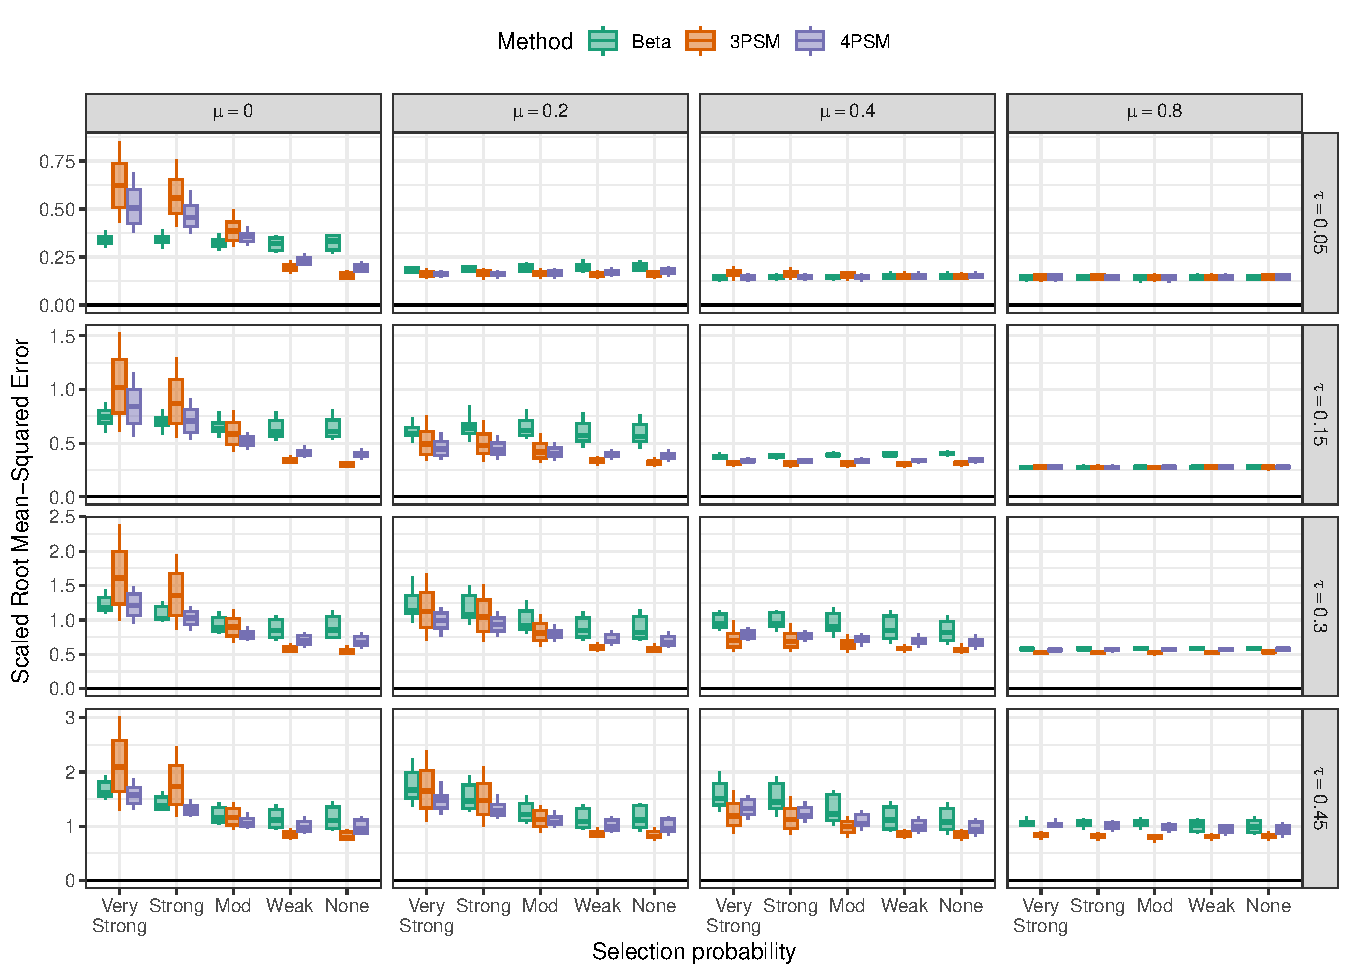
\includegraphics{simulation-results_files/figure-latex/mu-rmse-main-miss-1} \caption{Scaled root mean-squared error of the average effect size by method, selection probability, average SMD, and between-study heterogeneity}\label{fig:mu-rmse-main-miss}
\end{sidewaysfigure}

Figure (\textbf{ref?})(fig:mu-rmse-miss) presents the scaled RMSE for
the three selection models and highlights a clear bias--variance
trade-off. When average effect size is zero and selective reporting is
moderate to very strong, the results mirror the bias results pattern:
the beta-function selection model outperforms the step-function
selection models, and the 4PSM performs better than the 3PSM. However,
the relative performance shifts under other conditions. When average
effect size is \(\mu = 0.2\) and selective reporting is strong to very
strong, 4PSM yields the lowest RMSE. In contrast, when average effect
size is moderate or large (\(\mu \geq 0.2\)), or when \(\mu = 0.2\) and
selective reporting is absent to moderate, 3PSM outperforms both
alternatives. RMSE is similar across all models when average effect size
is moderate to large (\(\mu \geq 0.4\)) and heterogeneity is low
(\(\tau \leq 0.15\)).

\paragraph{Confidence Interval
Coverage}\label{confidence-interval-coverage-1}

\begin{Shaded}
\begin{Highlighting}[]
\NormalTok{mu\_graph\_res\_ci\_miss }\SpecialCharTok{\%\textgreater{}\%}
  \FunctionTok{filter}\NormalTok{(}
\NormalTok{    CI\_type }\SpecialCharTok{\%in\%} \FunctionTok{c}\NormalTok{(}\StringTok{"large{-}sample"}\NormalTok{)}
\NormalTok{  ) }\SpecialCharTok{\%\textgreater{}\%}
  \FunctionTok{ggplot}\NormalTok{(}\FunctionTok{aes}\NormalTok{(}\AttributeTok{x =}\NormalTok{ J, }\AttributeTok{y =}\NormalTok{ coverage, }\AttributeTok{color =}\NormalTok{ method, }\AttributeTok{fill =}\NormalTok{ method)) }\SpecialCharTok{+}
  \FunctionTok{geom\_boxplot}\NormalTok{(}\AttributeTok{alpha =}\NormalTok{ .}\DecValTok{5}\NormalTok{, }\AttributeTok{coef =} \ConstantTok{Inf}\NormalTok{) }\SpecialCharTok{+}
  \FunctionTok{geom\_hline}\NormalTok{(}\AttributeTok{yintercept =} \FloatTok{0.95}\NormalTok{, }\AttributeTok{linetype =} \StringTok{"dashed"}\NormalTok{) }\SpecialCharTok{+}
  \FunctionTok{coord\_cartesian}\NormalTok{(}\AttributeTok{ylim =} \FunctionTok{c}\NormalTok{(}\FloatTok{0.5}\NormalTok{, }\FloatTok{1.0}\NormalTok{)) }\SpecialCharTok{+} 
  \FunctionTok{scale\_y\_continuous}\NormalTok{(}\AttributeTok{expand =} \FunctionTok{expansion}\NormalTok{(}\FunctionTok{c}\NormalTok{(}\DecValTok{0}\NormalTok{,}\DecValTok{0}\NormalTok{),}\FunctionTok{c}\NormalTok{(}\FloatTok{0.02}\NormalTok{,}\DecValTok{0}\NormalTok{))) }\SpecialCharTok{+} 
  \FunctionTok{scale\_color\_brewer}\NormalTok{(}\AttributeTok{palette =} \StringTok{"Dark2"}\NormalTok{) }\SpecialCharTok{+}
  \FunctionTok{scale\_fill\_brewer}\NormalTok{(}\AttributeTok{palette =} \StringTok{"Dark2"}\NormalTok{) }\SpecialCharTok{+}
  \FunctionTok{facet\_grid}\NormalTok{(}
\NormalTok{    tau }\SpecialCharTok{\textasciitilde{}}\NormalTok{ mean\_smd, }
    \AttributeTok{labeller =} \FunctionTok{label\_bquote}\NormalTok{(}
      \AttributeTok{rows =}\NormalTok{ tau }\SpecialCharTok{==}\NormalTok{ .(tau),}
      \AttributeTok{cols =}\NormalTok{ mu }\SpecialCharTok{==}\NormalTok{ .(mean\_smd)}
\NormalTok{    ),}
    \AttributeTok{scales =} \StringTok{"free\_y"}
\NormalTok{  ) }\SpecialCharTok{+}
  \FunctionTok{labs}\NormalTok{(}
    \AttributeTok{x =} \StringTok{"Number of studies (J)"}\NormalTok{, }
    \AttributeTok{y =} \StringTok{"Coverage rate"}\NormalTok{, }
    \AttributeTok{color =} \StringTok{"Method"}\NormalTok{,}
    \AttributeTok{fill =} \StringTok{"Method"}
\NormalTok{  ) }\SpecialCharTok{+} 
  \FunctionTok{theme\_bw}\NormalTok{() }\SpecialCharTok{+}
  \FunctionTok{theme}\NormalTok{(}\AttributeTok{legend.position =} \StringTok{"top"}\NormalTok{)}
\end{Highlighting}
\end{Shaded}

\begin{sidewaysfigure}
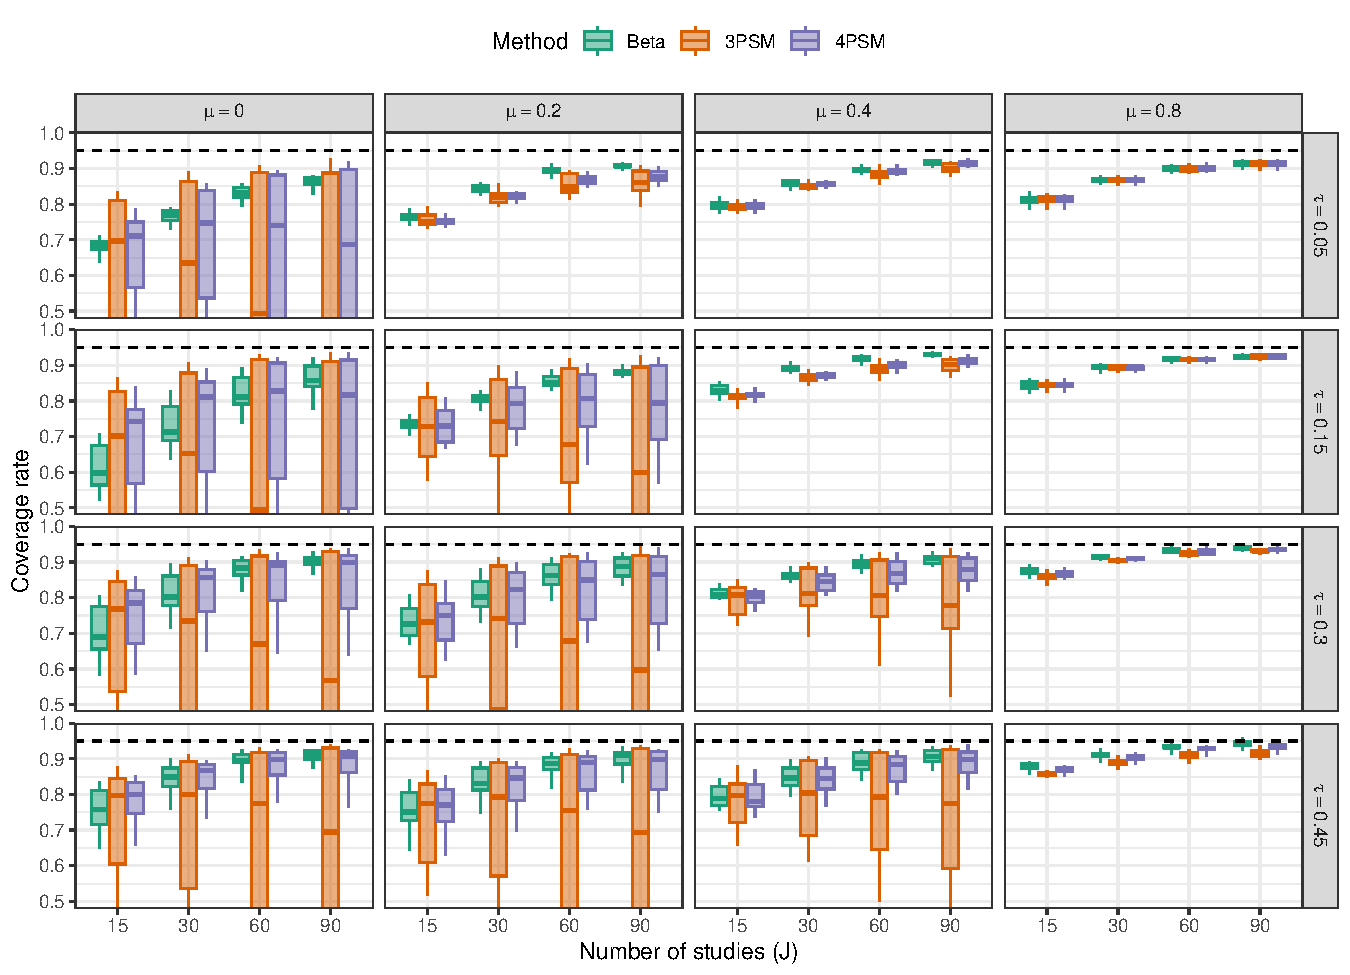
\includegraphics{simulation-results_files/figure-latex/comparison-coverage-miss-1} \caption{Coverage levels of confidence intervals for the average effect size based on cluster-robust variance approximations, by method, number of studies, average SMD, and between-study heterogeneity. Dashed lines correspond to the nominal confidence level of 0.95. Coverage rates of the 3PSM and 4PSM intervals are not depicted when they fall below 0.5}\label{fig:comparison-coverage-miss}
\end{sidewaysfigure}

Figure @ref(fig:comparison-coverage-miss) shows the coverage rates of
95\% confidence intervals based on large-sample cluster-robust variance
approximations for the three models\footnote{Once again, the vertical
  axis of Figure @ref(fig:comparison-coverage-miss) is restricted to the
  range {[}0.5, 1.0{]}, and coverage rates of the intervals based on
  3PSM and 4PSM are not depicted when they fall below 0.5. Supplementary
  Figure @ref(fig:comparison-coverage-full-miss) depicts the full range
  of coverage rates.} Coverage rates fall below the nominal 0.95 level
for all three selection models across most conditions. However, the
beta-function selection model generally achieves higher coverage than
the step-function selection models, particularly when heterogeneity is
moderate to large (\(\tau \geq 0.3\)), or when heterogeneity is low
(\(\tau \leq 0.15\)), average effect size is small (\(\mu \leq 0.2\)),
and number of studies (\(J\)) is 60 or more. As with CHE-ISCW and
PET/PEESE, the confidence intervals produced by the step-function
selection models are often miscalibrated, due in part to underestimated
standard errors, which result in overly narrow intervals. Among the
step-function selection models, coverage is generally higher for 4PSM
than for 3PSM.

\subsubsection{Effect Size Variance}\label{effect-size-variance}

\end{document}
